%%%%%%%%%%%%%%%%%%%%%%%%%%%%%%%%%%%%%%%%%
% Masters/Doctoral Thesis 
% LaTeX Template
% Version 2.5 (27/8/17)
%
% This template was downloaded from:
% http://www.LaTeXTemplates.com
%
% Version 2.x major modifications by:
% Vel (vel@latextemplates.com)
%
% This template is based on a template by:
% Steve Gunn (http://users.ecs.soton.ac.uk/srg/softwaretools/document/templates/)
% Sunil Patel (http://www.sunilpatel.co.uk/thesis-template/)
%
% Template license:
% CC BY-NC-SA 3.0 (http://creativecommons.org/licenses/by-nc-sa/3.0/)
%
%%%%%%%%%%%%%%%%%%%%%%%%%%%%%%%%%%%%%%%%%

%----------------------------------------------------------------------------------------
%	PACKAGES AND OTHER DOCUMENT CONFIGURATIONS
%----------------------------------------------------------------------------------------

\documentclass[
11pt, % The default document font size, options: 10pt, 11pt, 12pt
%oneside, % Two side (alternating margins) for binding by default, uncomment to switch to one side
english, % ngerman for German
singlespacing, % Single line spacing, alternatives: onehalfspacing or doublespacing
%draft, % Uncomment to enable draft mode (no pictures, no links, overfull hboxes indicated)
%nolistspacing, % If the document is onehalfspacing or doublespacing, uncomment this to set spacing in lists to single
%liststotoc, % Uncomment to add the list of figures/tables/etc to the table of contents
%toctotoc, % Uncomment to add the main table of contents to the table of contents
%parskip, % Uncomment to add space between paragraphs
%nohyperref, % Uncomment to not load the hyperref package
headsepline, % Uncomment to get a line under the header
%chapterinoneline, % Uncomment to place the chapter title next to the number on one line
%consistentlayout, % Uncomment to change the layout of the declaration, abstract and acknowledgements pages to match the default layout
]{MastersDoctoralThesis} % The class file specifying the document structure

\usepackage[utf8]{inputenc} % Required for inputting international characters
\usepackage[T1]{fontenc} % Output font encoding for international characters

\usepackage{mathpazo} % Use the Palatino font by default

\usepackage[backend=bibtex,style=numeric,natbib=true]{biblatex}
% was: backend=bibtex,style=authoryear,natbib=true
% Use the bibtex backend with the authoryear citation style (which resembles APA)

\addbibresource{references.bib} % The filename of the bibliography

\usepackage[autostyle=true]{csquotes} % Required to generate language-dependent quotes in the bibliography

%%%% added by me %%%%
\usepackage{bookmark, todonotes}
\newcommand{\missing}[1]{\textcolor{red}{#1}}

\graphicspath{{Chapters/Chapter03/figures/}{Chapters/Chapter04/figures/}}

\usepackage[cmex10]{amsmath}
\usepackage{graphicx}
\usepackage{hyperref}
\usepackage{subcaption}
\usepackage{stfloats}

%----------------------------------------------------------------------------------------
%	MARGIN SETTINGS
%----------------------------------------------------------------------------------------

\geometry{
	paper=a4paper, % Change to letterpaper for US letter
	inner=2.5cm, % Inner margin
	outer=3.8cm, % Outer margin
	bindingoffset=.5cm, % Binding offset
	top=1.5cm, % Top margin
	bottom=1.5cm, % Bottom margin
	%showframe, % Uncomment to show how the type block is set on the page
}

%----------------------------------------------------------------------------------------
%	THESIS INFORMATION
%----------------------------------------------------------------------------------------

\thesistitle{Security and Privacy of Blockchain Protocols and Applications} % Your thesis title, this is used in the title and abstract, print it elsewhere with \ttitle
\supervisor{Dr. Alex \textsc{Biryukov}} % Your supervisor's name, this is used in the title page, print it elsewhere with \supname
\examiner{} % Your examiner's name, this is not currently used anywhere in the template, print it elsewhere with \examname
\degree{Doctor of Philosophy} % Your degree name, this is used in the title page and abstract, print it elsewhere with \degreename
\author{Sergei \textsc{Tikhomirov}} % Your name, this is used in the title page and abstract, print it elsewhere with \authorname
\addresses{} % Your address, this is not currently used anywhere in the template, print it elsewhere with \addressname

\subject{Computer Science} % Your subject area, this is not currently used anywhere in the template, print it elsewhere with \subjectname
\keywords{} % Keywords for your thesis, this is not currently used anywhere in the template, print it elsewhere with \keywordnames
\university{\href{https://wwwen.uni.lu/}{University of Luxembourg}} % Your university's name and URL, this is used in the title page and abstract, print it elsewhere with \univname
\department{\href{https://wwwen.uni.lu/research/fstm/dcs}{Department of Computer Science}} % Your department's name and URL, this is used in the title page and abstract, print it elsewhere with \deptname
\group{\href{https://www.cryptolux.org/}{CryptoLUX Research Group}} % Your research group's name and URL, this is used in the title page, print it elsewhere with \groupname
\faculty{\href{https://wwwen.uni.lu/fstm}{Faculty of Science, Technology and Medicine}} % Your faculty's name and URL, this is used in the title page and abstract, print it elsewhere with \facname

\AtBeginDocument{
\hypersetup{pdftitle=\ttitle} % Set the PDF's title to your title
\hypersetup{pdfauthor=\authorname} % Set the PDF's author to your name
\hypersetup{pdfkeywords=\keywordnames} % Set the PDF's keywords to your keywords
}

\begin{document}

\frontmatter % Use roman page numbering style (i, ii, iii, iv...) for the pre-content pages

\pagestyle{plain} % Default to the plain heading style until the thesis style is called for the body content

%----------------------------------------------------------------------------------------
%	TITLE PAGE
%----------------------------------------------------------------------------------------

\begin{titlepage}
\begin{center}

\vspace*{.06\textheight}
{\scshape\LARGE \univname\par}\vspace{1.5cm} % University name
\textsc{\Large Doctoral Thesis}\\[0.5cm] % Thesis type

\HRule \\[0.4cm] % Horizontal line
{\huge \bfseries \ttitle\par}\vspace{0.4cm} % Thesis title
\HRule \\[1.5cm] % Horizontal line
 
\begin{minipage}[t]{0.4\textwidth}
\begin{flushleft} \large
\emph{Author:}\\
\href{https://s-tikhomirov.github.io/about/}{\authorname} % Author name - remove the \href bracket to remove the link
\end{flushleft}
\end{minipage}
\begin{minipage}[t]{0.4\textwidth}
\begin{flushright} \large
\emph{Supervisor:} \\
\href{https://www.cryptolux.org/index.php/Alex\_Biryukov}{\supname} % Supervisor name - remove the \href bracket to remove the link  
\end{flushright}
\end{minipage}\\[3cm]
 
\vfill

\large \textit{A thesis submitted in fulfillment of the requirements\\ for the degree of \degreename}\\[0.3cm] % University requirement text
\textit{in the}\\[0.4cm]
\groupname\\\deptname\\[2cm] % Research group name and department name
 
\vfill

{\large \today}\\[4cm] % Date
%\includegraphics{Logo} % University/department logo - uncomment to place it
 
\vfill
\end{center}
\end{titlepage}

%----------------------------------------------------------------------------------------
%	DECLARATION PAGE
%----------------------------------------------------------------------------------------
\iffalse % not seen in other theses in our group
\begin{declaration}
\addchaptertocentry{\authorshipname} % Add the declaration to the table of contents
\noindent I, \authorname, declare that this thesis titled, \enquote{\ttitle} and the work presented in it are my own. I confirm that:

\begin{itemize} 
\item This work was done wholly or mainly while in candidature for a research degree at this University.
\item Where any part of this thesis has previously been submitted for a degree or any other qualification at this University or any other institution, this has been clearly stated.
\item Where I have consulted the published work of others, this is always clearly attributed.
\item Where I have quoted from the work of others, the source is always given. With the exception of such quotations, this thesis is entirely my own work.
\item I have acknowledged all main sources of help.
\item Where the thesis is based on work done by myself jointly with others, I have made clear exactly what was done by others and what I have contributed myself.\\
\end{itemize}
 
\noindent Signed:\\
\rule[0.5em]{25em}{0.5pt} % This prints a line for the signature
 
\noindent Date:\\
\rule[0.5em]{25em}{0.5pt} % This prints a line to write the date
\end{declaration}
\fi

\cleardoublepage

%----------------------------------------------------------------------------------------
%	QUOTATION PAGE
%----------------------------------------------------------------------------------------

\vspace*{0.2\textheight}

\noindent\enquote{\itshape If you don’t believe it or don’t get it, I don’t have the time to try to convince you, sorry.}\bigbreak

\hfill Satoshi Nakamoto
% https://bitcointalk.org/index.php?topic=532.msg6306#msg6306

%----------------------------------------------------------------------------------------
%	ABSTRACT PAGE
%----------------------------------------------------------------------------------------

\begin{abstract}
\addchaptertocentry{\abstractname} % Add the abstract to the table of contents
This thesis explores various questions related to security and privacy of blockchain systems.

Bitcoin~\cite{nakamoto2008bitcoin} is a breakthrough system, allowing for the first time to transfer digital units of value without any trusted party.
Alternative cryptocurrencies inspired by Bitcoin aim at better addressing the issues of privacy, scalability, and feature set.
In particular, Ethereum introduces smart contracts in a Turing complete language and a stateful virtual machine, greatly expanding the design space of blockchain application, but expanding the attack surface as well.

% a part is a sequence of chapters
The first part of the thesis explores Ethereum.
Ethereum's expressive language, Solidity, provides lots of opportunities for developers to write insecure code.
We propose a simpler language based on Solidity, called Findel, to encode financial agreements in a more declarative fashion.
We study the vulnerabilities in real-world Ethereum contracts and present a tool that automates bug detection in Solidity using static analysis.
Finally, we describe a proposal to limit the privacy-damaging effects of existing legal requirements (know-your-customer, or KYC) if a financial service is implemented on top of Ethereum.

In the second part, we discuss the networking layer of Bitcoin and related cryptocurrencies.
We introduce an attack on privacy that allows an adversary to correlated transactions issued by the same user.
We test this technique on Bitcoin, as well as on the major privacy focused cryptocurrency.
We provide a separate overview of privacy-related functionality in mobile wallets.

The third part is dedicated to a promising approach at scaling blockchain, namely, off-chain protocols.
We study the Bitcoin's Lightning Network as the most prominent example of this approach.
We measure the potential effects of certain subset of Lightning nodes on privacy of the users.
Finally, we introduce a probing attack that lets an adversary reveal intermediary balances of payment channels it is not a part of -- the information supposed to be private.

\end{abstract}

%----------------------------------------------------------------------------------------
%	ACKNOWLEDGEMENTS
%----------------------------------------------------------------------------------------

\begin{acknowledgements}
\addchaptertocentry{\acknowledgementname} % Add the acknowledgements to the table of contents
\begin{itemize}
	\item advisor
	\item jury
	\item coauthors
	\item colleagues
	\item Uni staff, incl administrative
	\item Luxembourg
	\item Zcash foundation
	\item family
	\item Satoshi
\end{itemize}
\end{acknowledgements}

%----------------------------------------------------------------------------------------
%	LIST OF CONTENTS/FIGURES/TABLES PAGES
%----------------------------------------------------------------------------------------

\tableofcontents % Prints the main table of contents

\listoffigures % Prints the list of figures

\listoftables % Prints the list of tables

%----------------------------------------------------------------------------------------
%	ABBREVIATIONS
%----------------------------------------------------------------------------------------

\begin{abbreviations}{ll} % Include a list of abbreviations (a table of two columns)

\textbf{PoW} & \textbf{P}roof \textbf{o}f \textbf{W}ork\\
\textbf{LN} & \textbf{L}ightning \textbf{N}etwork\\

\end{abbreviations}

%----------------------------------------------------------------------------------------
%	PHYSICAL CONSTANTS/OTHER DEFINITIONS
%----------------------------------------------------------------------------------------

%\begin{constants}{lr@{${}={}$}l} % The list of physical constants is a three column table

% The \SI{}{} command is provided by the siunitx package, see its documentation for instructions on how to use it

%Speed of Light & $c_{0}$ & \SI{2.99792458e8}{\meter\per\second} (exact)\\
%Constant Name & $Symbol$ & $Constant Value$ with units\\

%\end{constants}

%----------------------------------------------------------------------------------------
%	SYMBOLS
%----------------------------------------------------------------------------------------

%\begin{symbols}{lll} % Include a list of Symbols (a three column table)

%$a$ & distance & \si{\meter} \\
%$P$ & power & \si{\watt} (\si{\joule\per\second}) \\
%Symbol & Name & Unit \\

%\addlinespace % Gap to separate the Roman symbols from the Greek

%$\omega$ & angular frequency & \si{\radian} \\

%\end{symbols}

%----------------------------------------------------------------------------------------
%	DEDICATION
%----------------------------------------------------------------------------------------

\dedicatory{For/Dedicated to/To my\ldots} 

%----------------------------------------------------------------------------------------
%	THESIS CONTENT - CHAPTERS
%----------------------------------------------------------------------------------------

\mainmatter % Begin numeric (1,2,3...) page numbering

\pagestyle{thesis} % Return the page headers back to the "thesis" style

% Include the chapters of the thesis as separate files from the Chapters folder
% Uncomment the lines as you write the chapters

% Chapter Template

\chapter{Introduction} % Main chapter title

\label{Chapter01_Introduction} % Change X to a consecutive number; for referencing this chapter elsewhere, use \ref{ChapterX}

This thesis explores security and privacy aspects of blockchains.

\part{Network-level privacy of Bitcoin and privacy focused cryptocurrencies}
% Chapter Template

\chapter{Introduction to P2P networks and their application to blockchains} % Main chapter title

\label{Chapter02_Intro_P2P} % Change X to a consecutive number; for referencing this chapter elsewhere, use \ref{ChapterX}

A peer-to-peer protocol is an essential part of a cryptocurrency.
The design goal of a cryptocurrency is open participation.
Every user must be able to verify the validity of the blockchain state.
Consequently, every user must be able to obtain the current state of the system from other peers.
\footnote{Zero-knowledge cryptography alleviates this requirement for some blockchain protocols.} % cite Coda

One of the design goals of ARPANET, the precursor to the Internet established in 1969, was reliability.
The network was designed to survive even if a large share of nodes were lost.
The key design decision enabling this was packet switching.
In contrast to earlier circuit switching networks, like the telephone network, where a dedicated end-to-end channel was assigned to any pair of currently connected parties, Internet protocols embrace the uncertainty stemming from connecting heterogeneous, geographically distributed computer networks.
Data is divided into packets, which are routed independently along various networks routes, to be re-combined at the receiving end.
No central server is responsible for routing: individual routers take decisions based on their view of the network.
This idea, counter-intuitive at the time, enabled the Internet to grow by many orders of magnitude, and still be resilient to disruptions.

As the Internet gained adoption with the general public in the 1990s, file-sharing networks emerged.
They allowed users to share large files very efficiently without relying on any one server.
The primary example of such networks is BitTorrent.
Over the years, it has shown impressive resiliency, surviving multiple attempts by law enforcement to shut individual BitTorrent trackers down due to them facilitating illegal content sharing.
Therefore it may be considered a precursor for Bitcoin.

BitTorrent resiliency remains an inspiration for cryptocurrency designers.
Satoshi Nakamoto, the creator of Bitcoin, wrote: "Governments are good at cutting off the heads of a centrally controlled networks like Napster, but pure P2P networks like Gnutella and Tor seem to be holding their own."~\cite{Nakamoto2008}.
\todo{Make an chapter or part epigraph?}
However, the goal of disseminating cryptocurrency data has important distinctions compared to file-sharing.

This introductory motivates our study of privacy issues of Bitcoin's P2P protocol and puts it in a historical context.
In~\ref{sec:C02_S1_Background_P2P}, we provide a historical overview of P2P networks and outline the similarities and differences in the functions of a file-sharing network and a P2P network powering a blockchain such as Bitcoin.
In~\ref{sec:C02_S2_Architecture_Bitcoin_P2P}, we describe the architecture of the networking layer of Bitcoin.
In~\ref{sec:C02_S3_Background_Wallets}, we describe the different types of cryptocurrency wallets.
Finally,~\ref{sec:C02_S4_Our_Contributions} puts our contributions, to be presented in detail in the following chapters of this part, into context.


\section{Background on P2P networks}
\label{sec:C02_S1_Background_P2P}

As any network, computer networks comprise of nodes.
An important question that network architects have to face is whether nodes are equal in their functions, or all nodes can perform the common set of tasks.

The former approach emphasizes efficiency.
We can draw an analogy with economic development of humanity, where the total wealth grows hand in hand with the division of labor.
Humans specialize in narrow tasks, getting very efficient at their professions, and exchange the fruit of their labor with others.
In network architecture, dedicating special nodes to perform operations such as coordination or data hosting brings efficiency.
Specialized nodes, can be implemented using optimized hardware (servers), maintained in specialized facilities (data centers) by professional technicians, take advantage of the economy of scale, and so on.

However, specialization harms resiliency.
If only a small group of people are responsible for a critically important set of functions, it only takes a relatively small number of them getting sick for adverse effects to propagate to the entire society.
In networking, likewise, if a dedicated group of servers maintains critical functions, it only takes one successful targeted attack, physical or by means of malware, to disrupt the whole network.

Keeping this trade-off in mind, let us review the development of P2P networks from file-sharing to blockchains.


\subsection{Early file-sharing networks}

The Internet has gained momentum in the developed world, with regular people and businesses exposed for the first time to the possibility of sharing data across the world with little to no pre-moderation.
Not surprisingly, the most common type of data people wanted to share media content such as movies and music.

File-sharing networks emerged in late 1990s to satisfy this demand, often by illegal means.
The two important early P2P networks are Napster and Gnutella~\cite{Gummadi2002}.
Napster -- the first successful music-centered file-sharing network -- was launched in 1999.
Having quickly gained millions of users, it drew attention from law enforcement, and was shut down in 2001.

An important point in the context of this thesis is that it was \textit{possible} to shut the network down.
Napster users were downloading content from each others' computers, but a central server was responsible for content search.
Without it, the network could not operate.

The Napster story emphasized the dilemma that P2P networks face.
In a file-sharing network, someone has to host the files.
If there is no central server, regular users must to this.
But regular users simply want to download a movie and watch it.
They do not want to take deliberate action "for the good of the network".
And as P2P network's value grows with the network effect, it is very important to make it simple for end users to use, but still make them contribute, maybe even without realizing it.

We can divide the task of file-sharing into two sub-tasks: locating a file and downloading it.
One nay argue that as long as a user knows where the required file is located, it is only a technical matter to download it efficiently.
A more crucial task, which Napster failed to implement in a resilient fashion, is content discovery.

Using a server for this task introduces a central point of failure and renders the network vulnerable.
Gnutella, on the other hand, went to the other extreme and used a flooding technique.
A user would forward the query to its neighbors, each of which would either reply with the requested content, or forward the query further.
While this approach has no single point of failure, it is significantly less efficient.


\subsubsection{BitTorrent}

BitTorrent~\cite{Pouwelse2005}, developed and launched in 2001, learned the lessons from both Napster and Gnutella.
Its design strikes a good balance between efficiency and resilience, without making user experience too unwelcoming.

As in other file-sharing P2P networks, users in BitTorrent download files from each other.
There are, however, multiple ways to locate the files.
One common way is \textit{torrent files}, which are distributed by specialized web servers -- \textit{trackers}.
A torrent file contains information about the file, its checksum, and addresses of some peers that likely host it.
This method does not make the whole network dependent on a single server, but a certain degree of centralization remains.
Alternatively, BitTorrent users may locate files with \textit{magnet links}, which utilize a modification of Kademlia~\cite{Maymounkov2002} -- a distributed hash table.

A distributed hash table (DHT) is a method of addressing content in a P2P network.
It randomly distributes content among nodes and allows for efficient querying.
It also requires only a minimal network restructuring when nodes leave or join.


\subsection{Incentives}

P2P file-sharing networks depended to a large extent on the users' goodwill.
They provided little monetary incentive for users to distribute files, let alone upload new content onto the network.
However, in contradiction to naive economical models, file-sharing networks gave birth to the \textit{warez scene} -- a community of people sharing content, mostly illegally, but with altruistic rather than profit-seeking motivations~\cite{Rehn2004}.
Regular users of file-sharing users were encouraged to share by trackers (in case of BitTorrent): for instance, by enforcing a ratio between what a user downloaded and uploaded.
However, such metrics are inherently vulnerable, as file-sharing network lack a strong identity system.
A tracker can force upload ratios for each account, but preventing users from signing up multiple times is tricky.
Protecting against such cheating -- Sybil attacks -- inevitably required an identity server, which would introduce a central point of failure.

Bitcoin solved the problem of Sybil protection in a decentralized network by using \textit{proof of work}.
\todo{Where should we introduce Bitcoin basics?}





\subsection{Design goals of a cryptocurrency P2P network}

BitTorrent remains the primary example of a computer network which no one was able to fully stop.
Despite multiple lawsuits against large torrent trackers, such as the Pirate Bay, as well as against regular users, law enforcers were unable to stop BitTorrent.
One may argue that this is impossible in principle: BitTorrent is just a protocol, in other words -- a language.
As long as the specifications are widely available, and there are two computers in the world willing to communicate according to its rules, BitTorrent is not dead.

This resiliency makes it similar to Bitcoin.
However, Bitcoin is not \textit{only} a set of rules -- it is a protocol that maintains specific \textit{state}.
While BitTorrent is agnostic to the format and semantics of the date being shared, Bitcoin's P2P layer is intended to share a concrete dataset -- the blockchain -- specific to the system at large.
This in the reason behind important distinctions between the design goals of a file-sharing networks (exemplified by BitTorrent for concreteness) and a cryptocurrency, exemplified by Bitcoin.


\subsubsection{Blockchain as a common dataset}

BitTorrent has no global state.
Users wishing to download a file join a \textit{swarm} of users who have (at least parts of) this file and have no interest in how other files are shared.

The goal of Bitcoin's P2P network is to share the single global state of the system.
The series of confirmed blocks contains the single source of truth on which key controls how many bitcoin.
Each user is interested in obtaining this dataset.
If Bob is expecting Alice to send him a payment for goods or services, he wants to make sure that she is not cheating.
To ensure that the received coins are genuine, Bob must check that they originate from a transaction in a confirmed block, and that transaction links back to another confirmed transactions, and so on, until the coinbase transactions that brought the coin to life by rewarding a miner.
Bob can only do so if he has the full dataset of all transactions that happened since the launch of the system.
(It is possible to get weaker assurances by performing simplified verification, but we omit these details for clarity.)

Sharing one global state means that content addressing is not a problem in Bitcoin.
There is no question about who has the required file, because every (full) node has it.
However, Bitcoin nodes generally do not want to get eclipsed.
\todo{Move to own subsubsection?}





\subsubsection{Logical properties of blockchain data}

BitTorrent is agnostic to the semantics or format of the files being shared.
In Bitcoin, the data has a logical order.
Each block depends on the previous block.
A Bitcoin node (assuming the most conservative threat model) should download the blockchain sequentially, verifying every block.


\subsubsection{Timing requirements}

BitTorrent file-sharing is process bounded in time: a user downloads a file, and leaves the network.
In contrast, cryptocurrency P2P networks perform constant synchronization, as new transactions and block are being generated.

\todo[inline]{IBD vs keeping in sync; miners vs non-miners}


\subsubsection{Incentives and privacy}

BitTorrent seeders are not incentivized by the protocol itself.
\todo{search J. Backus twitter for links to P2P papers on this}
While the protocol accounts for the actual bandwidth and assigns a higher internal weight to peer with fast and reliable connections, such in-protocol points are hard to convert into more conventional value systems.
Some torrent trackers employ reputation systems, where the tracker gives additional privileges to active seeders, but torrent seeders have been largely altruistic.

Bitcoin, on the contrary, is powered by economic incentives.
Nevertheless, sharing blockchain data is not incentivized directly.
Nodes get no reward for propagating data to their peers.
As BitTorrent has shown, this may be sufficient to provide \textit{availability}, but it is not clear whether is also enables \textit{integrity}.

In file-sharing, nodes seldom have incentives to lie.
Notwithstanding rare examples of "poisoned torrents", BitTorrent users get the content they expect.
In cryptocurrencies, propagating false data may be a part of an attack.
An adversary eclipsing a victim with nodes under their control may make them believe that a different state of the blockchain is valid, compared to what the larger world is agreeing upon.
To prevent this, Bitcoin and other cryptocurrencies deliberately choose neighbors randomly from a large set of possibly live nodes, and additional checks ensure network diversity among one's neighbors.

Privacy (and fungibility as a result) is a crucial property of money.
The lack of privacy in BitTorrent enabled tracking its users.
% https://www.vice.com/en_us/article/d3q45v/bittorrent-usage-increases-netflix-streaming-sites
Bitcoin provide little privacy both on the application layer (the transaction graph) and on the networking layer.
\todo{Is this really different?}






\section{Architecture of Bitcoin P2P layer}
\label{sec:C02_S2_Architecture_Bitcoin_P2P}

In this Section, we describe the architecture of Bitcoin's networking protocol.

\section{Background on cryptocurrency wallets}
\label{sec:C02_S3_Background_Wallets}

In this Section, we give a background on the types of cryptocurrency wallets and the trade-offs their developers and users face.


\section{Our contributions}
\label{sec:C02_S4_Our_Contributions}

As outlined in~\ref{sec:C02_S2_Architecture_Bitcoin_P2P}, there are two vectors of attacks on privacy: local and global.

\chapter{Deanonymization of cryptocurrency transactions with network analysis} % Main chapter title

\label{Chapter03_Clustering}

We present a novel technique to analyze the public traffic in a P2P network of Bitcoin and other cryptocurrencies and extract information about the senders of transactions.
% Chapter Template

\chapter{Privacy of cryptocurrency wallets} % Main chapter title

\label{Chapter04_Wallets} % Change X to a consecutive number; for referencing this chapter elsewhere, use \ref{ChapterX}

In this chapter, we review the privacy-related aspects of cryptocurrency wallets for Android.

\part{Privacy of the Lightning Network}
% Chapter Template

\chapter{Introduction to Lightning Network} % Main chapter title

\label{Chapter05_Intro_Lightning} % Change X to a consecutive number; for referencing this chapter elsewhere, use \ref{ChapterX}

We present an introduction to the second layer (L2) blockchain protocols and in particular the Lightning network for Bitcoin.
\chapter{Probing Lightning channel balances}

\label{Chapter06_LN_probing}

We describe a technique for cheaply and quickly probing intermediate balances of Lightning channels -- information which is considered private.
% Chapter Template

\chapter{Quantitative analysis of Lightning network privacy} % Main chapter title

\label{Chapter07_LN_attacks} % Change X to a consecutive number; for referencing this chapter elsewhere, use \ref{ChapterX}

We evaluate the possibility of various attacks on Lightning, considering various subsets of nodes potentially compromised.
\chapter{Throughput limitation of the Lightning network}

\label{Chapter08_HTLC_limit}

We describe an inherent limitation on the number of concurrent payments Lightning channels can handle.

\part{Security of smart contracts on Ethereum}
\chapter{Introduction to secure programming and smart contracts}

\label{Chapter09_Intro_contracts}

We introduce the notion of smart contracts along with the history of approaches to secure programming practices in general.
\chapter{Findel: Secure derivative contracts for Ethereum}

\label{Chapter10_Findel}

We introduce a declarative language for financial derivatives on top of Solidity.
% Chapter Template

\chapter{SmartCheck: Static analysis of Ethereum smart contracts} % Main chapter title

\label{Chapter11_SmartCheck} % Change X to a consecutive number; for referencing this chapter elsewhere, use \ref{ChapterX}

We present SmartCheck -- a static analysis tool for smart contracts in Solidity.
\chapter{Privacy-preserving KYC on Ethereum}

\label{Chapter12_KYC}

We present a scheme which allows for a development of an Ethereum based token usable only to white-listed entities while preserving their privacy.

Identity is a fundamental concept for the financial industry.
In order to comply with regulation, financial institutions must verify the identity of their customers.
Identities are currently handled in a centralized way, which diminishes users' control over their personal information and threats their privacy.
Blockchain systems, especially those with support for smart contracts (e.g.,~Ethereum), are expected to serve as a basis of more decentralized systems for digital identity management.

We propose a design of a privacy-preserving KYC scheme on top of Ethereum.
It would let providers of financial services leverage the potential of blockchain technology to increase efficiency of customer onboarding while complying with regulation and protecting users' privacy.


%%%%%%%% SECTION 1. Introduction %%%%%%%%

\section{Introduction}

Digital identity is information used by a computer system to represent a user.
It serves two purposes:

\begin{itemize}
	\item Authentication: to prove that the user is who they claim to be;
	\item Authorization: to ensure that the user has the right to perform the action they are trying to perform.
\end{itemize}

Modern financial system adheres to the centralized identity model and depends on government-issued identities.
Regulation in most jurisdictions demand that banks obtain proof of identity from customers before doing business with them ("know your customer", or KYC).
"Anti money laundering" (AML) and "counter terrorist financing" (CTF) are related regulations that require banks to stop and report suspicious transactions.
%In financial services,  and privacy violation can lead to serious consequences.

Modern KYC is not only cumbersome but also privacy violating.
Users' sensitive information is stored in banks' databases, where it is difficult to update and can be stolen by corrupt employees or external hackers.
Banks implement KYC/AML procedures independently, which leads to high compliance cost for the industry as a whole, as well as multiplies the risk of identity theft and privacy violations.

Open blockchains, the first one being Bitcoin, take a different approach to identity: users join the network without any identification.
This technology enabled the creation of more sophisticated decentralized networks with rich programming capabilities, e.g.,~Ethereum.
Banks and other financial services companies see the potential of blockchain technology and are collaborating on its applications in consortia such as Enterprise Ethereum Alliance~\cite{EEA2017}, Hyperledger~\cite{Hyperledger}, and R3~\cite{R3}.
Though to comply with regulation, they have to handle government-issued identities in a blockchain setting, which is a non-trivial task.
Taking into account the users' demand for better privacy protection, this becomes even harder.
The upcoming European privacy regulation (GDPR~\cite{GDPR16}) coming into force in May~2018 poses even more challenges for organizations that handle users' personal data.

We first explore the centralized and decentralized approaches to identity.
We then propose KYCE -- a privacy preserving Ethereum-based KYC implementation for smart contract based financial services.
KYCE allows banks to implement KYC checks via an external smart contract -- a KYC provider.
Our scheme uses zero-knowledge proofs to check users' eligibility without disclosing their private information to anyone except the KYC provider.
The whitelist is stored in the KYC smart contract in the form of a cryptographic accumulator.
This construction allows users to be efficiently added to, removed from, and checked against a list without storing any plaintext data on the blockchain.
We then discuss possible use cases, implementation challenges, and outline the direction for future work.

\subsection{Centralized identity}

We can re-formulate the notion of identity in terms of asymmetric cryptography.
Identity $I$ of user $U$ is a public-private key pair $(pub_U, priv_U)$.
The public key $pub_U$ authenticates the user (or, equivalently, links the current action to some past actions).
Public identifiers like username or address are derived from $pub_U$.
The private key $priv_U$ allows $U$ to sign messages on behalf of $I$.
From the point of view of the system, $U$ is whoever possesses $priv_U$.

In the centralized model of identity, which is prevalent on the internet today, users delegate managing their private keys to a trusted party and use a password to access them when necessary.
This approach is sub-optimal in many regards.
First of all, users do not control their identities.
The trusted party always has the technical ability to sign messages without the user's consent or to prevent the user from signing the message they want.
Moreover, users' personal data is stored by a centralized entity, which creates additional incentives for malicious actors to attack it.
Finally, users have to create a new identity for each website they wish to register with.
As a consequence, they adhere to a risky practice of reusing passwords.
This problem is partially addressed with the "login with" feature, often implemented using protocols such as OAuth and OpenID~\cite{Dodanduwa2018}.
In this scheme, a third-party website queries the website that holds the user's existing identity (e.g.,~Google) and asks for permission to access a subset of the user's data (e.g.,~name and email).
Upon approval, the access is granted.
This approach alleviates the password management problem but increases the impact of a potential identity theft.

Even though users can revoke the access at any time, the "login with" scheme is still privacy violating.
Imagine a user that reveals their date of birth to prove to a website that they are 18 years of age or older.
Even if they later revoke the access, their date of birth will never change.
Thus, they grant the third-party website an effectively unlimited access to a piece of private information.

Maintaining correspondence between "real world" identities and public keys has long been a challenge.
Centralized solutions like PKI generally work, but suffer from risks associated with centralization: a fraudulent authority can issue rogue certificates~\cite{Amann2017}.


\subsection{Decentralized identity and open blockchains}

A noteworthy approach to decentralized identity is the PGP "web of trust"~\cite{Feisthammel2017}.
It has not gained significant traction due in part to usability challenges~\cite{Ruoti2015} and concerns about the security of the long-term key model~\cite{Valsorda2016}.

Bitcoin~\cite{Nakamoto2008} is the first practical implementation of fully decentralized digital cash.
It eliminates the problem of connecting public keys to identities in a radical manner: in Bitcoin, public keys \textit{are} identities.
Since its launch in 2009, hundreds of alternative open blockchains were developed, most of them adhering to this approach to identity management.

Ethereum~\cite{Buterin2014, Wood2014} is a decentralized blockchain-based smart contracts platform.
Smart contracts were initially defined as "a set of promises, specified in digital form"~\cite{Szabo1996}.
In Ethereum, a smart contract is a piece of code in Ethereum virtual machine (EVM) bytecode, a Turing complete language.
Programmers write contracts in high-level languages targeting EVM, most popular being Solidity, and deploy them onto the blockchain.
Users interact with contracts by broadcasting transactions.
Upon receiving a transaction, Ethereum nodes execute the corresponding function of the specified contract with given arguments.
Nodes maintain a common view of the state using a proof-of-work consensus mechanism.

Contracts can call other contracts' functions and send them units of the Ethereum native cryptocurrency \textit{ether}.
Each EVM operation has a cost denominated in units of \textit{gas} to prevent denial-of-service attacks.
The user determines the maximum amount of resources their computation will consume and pays for it upfront when sending the transaction.
If the computation executes normally, the user gets a refund for the remaining gas.
In case of an exception, all allocated gas is consumed, but the transaction has no effect on the state of the blockchain\footnote{After the Byzantium update in October~2017, certain types of exceptions no longer consume all gas.}.

%See~\cite{Allen16} on the evolution of identity from centralized to self-sovereign.

Traditional financial institutions are becoming interested in blockchain technology, especially in networks enabling smart contracts~\cite{Castillo2017}.
However the way open blockchains handle identity may come at odds with financial regulation.
We propose a design that will simultaneously leverage the power of blockchain-based smart contracts, enable banks to implement KYC to comply with the law, and preserve users' privacy.


\subsection{Financial and privacy regulation in the EU} \label{sec:Ch12_KYC_EU}

The current EU legislation "on information accompanying transfers of funds" came into effect in 2015~\cite{EU847}.
In the wake of the rapid growth of cryptocurrencies, the EU is tightening its \textbf{anti-money laundering regulations}, stating that "virtual currency exchange platforms and custodian wallet providers will have to apply customer due diligence controls, ending the anonymity associated with such exchanges"~\cite{EU16}.
Vandezande analyzes virtual currencies under the EU anti-money laundering law~\cite{Vandezande2017}.

2018 is set to be a "game-changing" year for European financial industry, as two important regulations come into force.

The \textbf{Revised Payment Service Directive} (PSD2) obligates banks to provide third-party providers access to their customers' accounts through open APIs~\cite{Hellstroem2017}.
This is meant to foster competition and give rise to third-party financial service providers.
For instance, unified banking API will likely make connecting banks' infrastructure to open blockchains simpler~\cite{Elison2016}.

The \textbf{General Data Protection Regulation} (GDPR), coming into force on 25~May~2018, harmonizes data privacy laws across the EU~\cite{GDPR16} and introduces stricter rules for handling data of EU residents even for companies from outside the EU.
Berberich and Steiner describe possible implications of blockchain adoption from the point of view of the EU data protection regulation~\cite{Berberich2016}.

%%%%%%%% SECTION 2. KYCE %%%%%%%%


\section{KYCE: a decentralized KYC-compliant exchange}

\subsection{Definitions and security properties}

KYC requirements differ depending on jurisdiction~\cite{PWC2015} (see Section~\ref{sec:Ch12_KYC_EU} for a brief overview of the regulatory landscape in the EU).
A typical KYC procedure links users' real-world identities to their accounts and checks users against a whitelist or a blacklist.
The details of the KYC procedure do not affect our design.

\begin{definition}
	A \textbf{KYC procedure} is a process that determines if a given user is eligible for a given transaction.
\end{definition}

\begin{definition}
	A \textbf{KYC provider} is an entity that performs a KYC procedure.
\end{definition}

\begin{definition}
	A \textbf{financial service} is an information system that allows users to exchange units of value.
\end{definition}

\begin{definition}
	A financial service is \textbf{KYC-compliant} w.r.t. the KYC procedure iff all users are eligible for all transactions they perform.
\end{definition}

\begin{definition}
	A KYC-compliant financial service is \textbf{privacy-preserving} iff only the KYC provider has access to the users' private data.
\end{definition}


\subsection{Tokens and exchanges}

Our KYC solution can be applied for any type of service.
For concreteness, consider a token exchange as an example of a financial service.

\begin{definition}
	A \textbf{token} is a transferable fungible unit of value maintained by a smart contract.
\end{definition}

ERC20~\cite{Victor2019} is the de-facto standard API for implementing token contracts in Ethereum.
A token contract keeps track of users' token balances and enables them to transfer tokens using the following functions:

\begin{itemize}
	\item \texttt{transfer} sends a given amount of tokens to a given address.
	\item \texttt{approve} allows a given user to withdraw up to a given amount of tokens from the account of the user calling the function.
	\item \texttt{transferFrom} sends a given amount of tokens from one given address to another (the amount has to be \texttt{approve}d beforehand).
\end{itemize}

\begin{definition}
	An \textbf{exchange} is a service that enables users to exchange tokens.
\end{definition}

The most prevalent type of exchanges is centralized ones, implemented as a regular web service.
In this work, we are mostly interested in decentralized, or on-chain exchanges, implemented as smart contracts. 

An exchange without KYC support may be used as follows.
\begin{enumerate}
	\item Alice creates an order to sell $X$~A-tokens for $Y$~B-tokens.
	\item Bob creates an order to sell $Y$~B-tokens for $X$~A-tokens.
	\item The exchange matches the two orders and transfers (by calling \texttt{transferFrom}) $X$~A-tokens from Alice to Bob and $Y$~B-tokens from Bob to Alice.
\end{enumerate}

The transaction succeeds if Alice and Bob \texttt{approve}d the exchange with sufficient amount of A- and B-tokens respectively before \texttt{transferFrom} is called.
Users withdraw tokens from the exchange by calling \texttt{approve(exchangeAddress,0)}.



\subsection{Privacy-preserving KYC}

We propose KYCE -- a privacy-preserving KYC design for Ethereum-based financial services.

A KYC contract provides an API to other contracts so that external services can determine if a given user is KYC-approved for using a given token.
A KYC provider (a governmental entity or company in charge of customer onboarding) performs the necessary checks for a new customer and adds their address to the whitelist.

A naive approach to implementing KYC check with a separate contract would be the following.
The KYC contract stores the whitelist of approved addresses.
On every \texttt{transfer}, token contracts check if the address which is being used belongs to the whitelist.
This design has a fundamental drawback from the privacy-preserving standpoint: all whitelisted addresses are stored on the blockchain in plaintext.
Moreover, users must use the same addresses they registered with the KYC provider, which violates privacy: an adversary can link the user's transactions in the public blockchain.

\paragraph{Our approach}
We use cryptographic techniques to design a privacy preserving KYC solution.
In KYCE, the KYC contract stores a \textbf{cryptographic accumulator} of the whitelisted addresses. 

A cryptographic accumulator $A$ absorbs certain algebraic objects and provides an interface to generate and verify zero-knowledge proofs that a certain value was accumulated.
In our construction, to generate a proof for value $x\in A$ one needs a \emph{witness}, which depends on $A$ and $x$ and is provided by the accumulator owner to the user who submitted $x$.
We suggest an accumulator based on bilinear maps due to Camenisch et al.~\cite{Camenisch2009}.

Briefly, the KYC setup and workflow is as follows.
The KYC provider creates and publishes a smart contract, which is initialized with an empty accumulator.
The User interacts with the KYC provider physically or online and provides credentials needed to pass the KYC procedure.
He also generates his own master secret $m$ and during the authenticated session gives the provider a Pedersen commitment $g_1^m\cdot g_2^r$ to it, where $g_1,g_2$ are certain group generators\footnote{Here and in the further text all
	multiplications take place in the pre-selected group of prime order $q$, typically an elliptic-curve group.} and $r$ is random.
If the checks are passed, the provider updates the accumulator with user-dependent data and provides the User with a witness, needed to prove the KYC property in the future.
In every Ethereum transaction to KYCE, the User provides a proof that he has been registered in the accumulator, that his right has not been revoked, and that the proof owner and the transaction sender are the same person.
The latter statement is verified by KYCE, whereas the rest is submitted to the KYC contract for verification against the current accumulator value.
If the checks pass, the command is executed in KYCE.

\paragraph{Details on the accumulator construction} We follow the approach by Camenisch et al.~\cite{Camenisch2009}, who construct an accumulator based on a pairing function $e(\cdot,\cdot)$ in some pairing setting~\footnote{The original paper~\cite{Camenisch2009} uses type-1 pairings, but type-3 pairings can be adopted as well.}.
The accumulator contains just serial numbers, possibly consecutive integers\footnote{It is possible to store public keys but it would be less efficient.}.
The accumulator is constructed as follows.
We assume a bilinear pairing $e:\,G\times G\rightarrow G_T$ where 
$G,G_T$ are groups of order $q$. The KYC provider selects generator $g$ and the secret value  
$\gamma\overset{\$}{\leftarrow} \mathbb{Z}_q$. It also selects $L$ as an upper bound of users enabled for KYC  and computes $z = e(g,g)^{\gamma^{L+1}}$. The accumulator value
$\mathrm{A}$ is initialized by $1$. 

Let us denote $g_i = g^{\gamma^i}$.
The provider publishes
$\mathrm{A},\{g_i\}_{1\leq i\leq L, \,L+2\leq i \leq 2L}$, the set of registered KYC indices $V=\emptyset$, and the parameters $g,z$ needed 
to perform a verification.

Every User who passes the KYC check is issued a new serial number $i$, the witness $w_i = \prod_{j\in V,j\neq i} g_{L+1-j+i}$, where $V$ is the set of all issued serial numbers, and a signature $\sigma_i$ of $g_i||i$ on the provider's private signature key.
The witness is used to generate a proof of accumulating\footnote{We refer an interested reader to \cite{Camenisch2009} for the details.}.
The accumulator is updated by the KYC provider with $i$ by 
$$
\mathrm{A_{V\cup\{i\}}} \leftarrow \mathrm{A_V} \cdot g_{L+1-i}
$$multiplying it by $g_{L+1-i} = g^{\gamma^{L+1-i}}$, and $i$ is published as a new valid serial number.
To prove that $i$ has been committed to $A$ and has not been revoked without disclosing it, the holder of $w_i$ must update it\footnote{We omit the details, but the update can be performed just before the presentation, not necessarily after every accumulator update.} so that the 
following equation holds:
$$
\frac{e(g_i, A)}{e(g,w_i)} = z.
$$

Note that revocation is also efficient: the KYC contract owner simply multiplies the accumulator value by the inverse of $g_{L+1-i}$. The witness value can not be updated anymore.

\paragraph{Presentation} 
When issuing a transaction to use the exchange (e.g.,~create an order), the user submits a \textbf{zero-knowledge proof} of the following statement:
\begin{itemize}
	\item I know the private key of the current user address (\texttt{msg.sender}), and
	\item I know a signature $\sigma_i$ and a witness $w_i$ for some number $i$ that has been accumulated in the
	accumulator $A$ in the KYC contract.
\end{itemize}
It is crucial that this compound statement is \emph{atomic}, i.e. the sub-statements can not be extracted
as separate valid proofs, as this would make the transaction malleable.

The atomicity (and thus non-malleability) are ensured as follows. Let us denote the
proof of knowledge for the witness and signature by $PK_w$, which is given in~\cite{Camenisch2009}, Section 4.2. Then Prover submits 
$$
P = \{PK_w \wedge PK_s\},
$$
where $PK_s$ is the proof of knowledge of the private key of the \texttt{msg.sender}'s ECDSA public key, which can be taken from~\cite{Chase2016}. The technique to make a composite proof of knowledge is straightforward as both PoKs are non-interactive and is standard in complex PoK protocols:
\begin{enumerate}
	\item Prover collects a set $\mathcal{C}$ of commitments 
	asserted in sub-proofs $PK_w$ and $PK_s$.
	\item Prover makes necessary randomization of $\mathcal{C}$ to create $t$-values $\mathcal{T}$.
	\item Prover computes $c \leftarrow H(\mathcal{C},\mathcal{T})$.
	\item Prover computes $s$-values  $\mathcal{S}$ using
	$\mathcal{C}$,  $\mathcal{T}$, and $c$.
	\item The proof $P$ is $(\mathcal{C}, \mathcal{S},c)$.
	To verify it one computes asserted $t$-values $\widehat{\mathcal{T}}$ and verifies
	$$
	c\overset{?}{=}H(\mathcal{C},\widehat{\mathcal{T}}).
	$$
\end{enumerate}

The resulting proof $P$ is submitted as an Ethereum transaction argument.
KYCE retrieves the most recent accumulator value and verifies $P$ against it and the public key of the message sender, which is available in the transaction metadata.
If the proof is correct the order is executed.


\subsection{Use cases}

Either the exchange contract or the token contract must be KYC-compliant -- i.e.,~check eligibility of transacting parties using the implementation of the cryptographic scheme described above in the KYC contract.

\paragraph{KYC-compliant exchange}

If the exchange is KYC-compliant, the tokens do not need to be aware of the KYC.

\begin{figure}[h]
	\caption{KYC-compliant exchange}
	\centering
	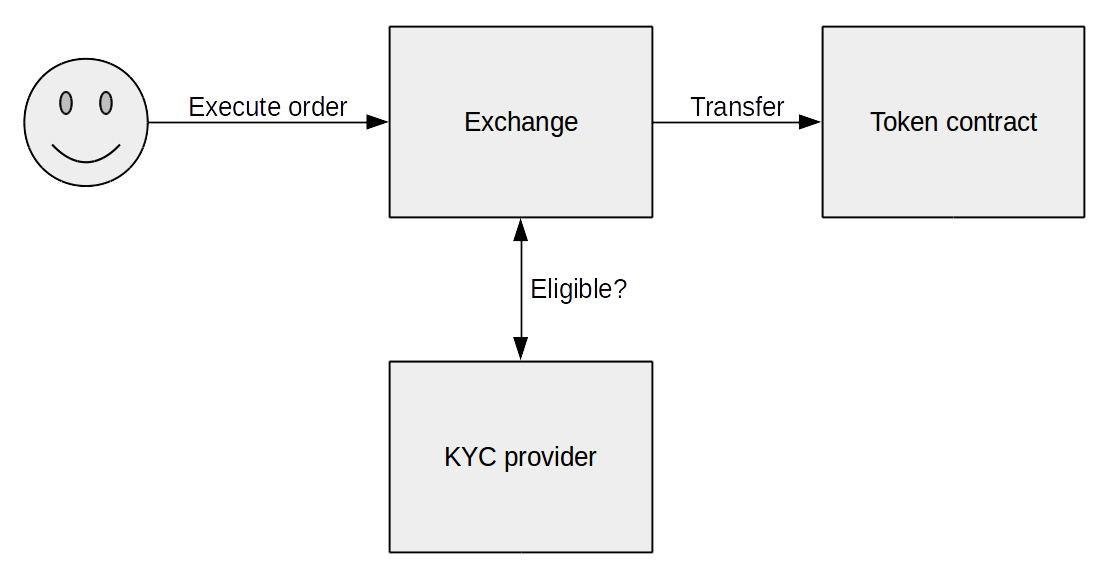
\includegraphics[width=0.45\textwidth]{figure-kyc-exchange}
\end{figure}

Consider an established exchange that trades dozens of tokens.
It applies for official approval in a jurisdiction that requires all customers to pass the KYC procedure.
The governmental body acts as a KYC provider, deploys a KYC contract, and publishes its address.
The exchange adds KYC checks to its codebase and continues operation.
Users who do not want to apply for KYC can simply withdraw their tokens from the exchange and use them elsewhere.


\paragraph{KYC-compliant token}

If the token is KYC-compliant, the exchange does not need to be aware of the KYC.

\begin{figure}[h]
	\caption{KYC-compliant token}
	\centering
	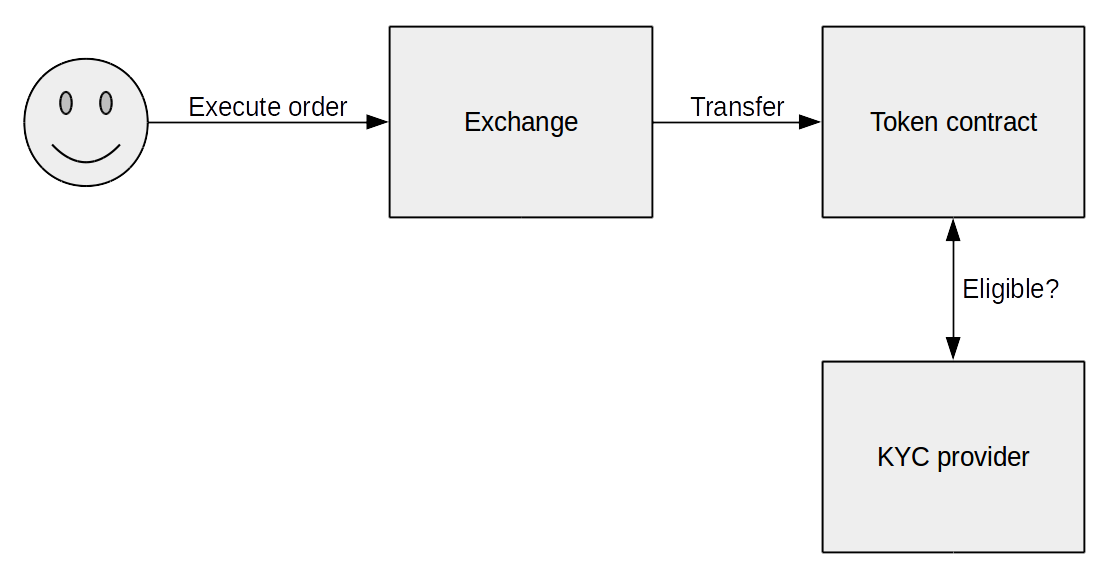
\includegraphics[width=0.45\textwidth]{figure-kyc-token}
\end{figure}

Consider a government that issues its own tokens\footnote{Bank of England~\cite{Danezis2016} and the Monetary Authority of Singapore~\cite{Singapore17} already did research in this direction.}.
Government tokens could be used by KYC-approved users for tax payments, fees, fines, etc.
Such solution leverages the flexibility and auditability of smart contracts while limiting the userbase of the token to the approved entities only.
The KYC-enabled government token can be also traded on exchanges.
This allows citizens to hold their wealth in currency portfolios of their choice and only purchase government tokens to transact with the state.

\paragraph{Transaction-dependent checks}

Many jurisdictions impose additional restrictions that depend on the value of the transaction.
E.g.,~the EU regulation~\cite{EU847} states that "the obligation to check whether information on the payer or the payee is accurate should [...] be imposed only in respect of individual transfers of funds that exceed \EUR{1000}".
EU member states impose further restrictions for transactions of higher value, e.g.,~exceeding \EUR{10000} in Belgium, \EUR{15000} in Germany and in the Netherlands~\cite{PWC2015}.
Either the exchange contract or the token contract can perform such checks by storing the following mappings:
\begin{itemize}
	\item address $=>$ accumulated transaction volume in the current period (day, month, year);
	\item address $=>$ timestamp of the latest transaction. 
\end{itemize}



%%%%%%%% SECTION 3. Implementation details %%%%%%%%

\section{Implementation details}

We created a proof-of-concept implementation of the proposed design.
Our project consists of two smart contracts written in Solidity: KycProvider and KyceToken.
% TODO: add link to Github

\subsection{Initial (not privacy-preserving) implementation}
In the initial (not privacy-preserving) implementation, KycProvider maintains a 2-dimensional boolean array that stores the eligibility status across users and tokens.
On initialization, the address that deploys the contract to the blockchain is made the \textit{owner}, allowing it to add and remove users from the array.
The ownership may be transferred (using the functionality inherited from the standard Ownable contract).

The KycProvider exposes the following API:

\begin{itemize}
	\item \texttt{add(address \_user, address \_token)} -- makes the user eligible for using the token (callable only by the owner)
	\item \texttt{remove(address \_user, address \_token)} -- makes the user not eligible for using the token (callable only by the owner)
	\item \texttt{isEligible(address \_user, address \_token)} -- checks if the user is eligible for using the token
\end{itemize}

KyceToken adheres to the de-facto standard token API in Ethereum -- ERC20.
To minimize the risk of security issues due to implementation subtleties, we inherit a widely used and tested ERC20 implementation by OpenZeppelin.
We override the functions \texttt{approve}, \texttt{transfer}, and \texttt{transferFrom} to check if the given user (\texttt{msg.sender}) is eligible for using this token.
Namely, the function \texttt{isEligible} is called.
If the returned value is \texttt{false}, the execution stops; is it is \texttt{true}, the corresponding function of the super class is invoked.

The implementation of the proposed scheme requires cryptographic primitives partially already available in Ethereum as pre-compiled contracts (namely, elliptic curve addition and scalar multiplication, as well as pairing checks).
For the proposed scheme to be fully implemented, pairing evaluation is also required.
We are looking into the possibilities to add this functionality.


%%%%%%%% SECTION 4. Related work %%%%%%%%

\section{Related work}

Parra-Moyano and Ross use distributed ledger technology to improve the KYC process~\cite{Moyano2017}.
Their proposal can be summarized as follows:
\begin{itemize}
	\item the regulator maintains a database with all users' private data;
	\item the first bank a user signs a contract with (the "home bank") stores hashes of the user's documents in a smart contract in a permissioned blockchain;
	\item all subsequent banks the user wants to work with obtain the user's documents from the database and look the hash up to ensure that the user had been KYC-approved (without knowing which home bank had done it);
	\item a cost-sharing mechanism for banks allows to proportionally share the cost of the initial KYC approval among all banks that use it.
\end{itemize}
In this design, all banks store users' private data -- contrary to our solution, where it is stored only with the KYC provider.
A more decentralized design is also proposed, but the authors claim it to be of a lesser practical relevance.

Sullivan and Burger investigate possible implications of further development of the Estonian e-residency program using blockchain technology~\cite{Sullivan2017}.
E-residency of Estonia is a governmental program that provides applicants with a digital identity, which can then be used, e.g.,~to register a company and open a bank account.
Estonian e-residency disconnects a digital identity from citizenship or physical residence.
Within the e-residency program, Estonia collaborates with a blockchain project Bitnation~\cite{Bitnation15, Estonia15}.
Oraclize, a company that provides trusted external data to Ethereum smart contracts, implemented a connector that lets Ethereum contracts handle e-residency identities~\cite{Provable}.

An existing project~\cite{Ohtamaa2016} implements a KYC scheme in an Ethereum smart contract, but stores the KYC status on the blockchain in plaintext.

There are multiple projects aimed at easing customer onboarding (creating an identity for a new user and ensuring KYC compliance) for banks.
Some of the projects are: Cambridge Blockchain~\cite{CambridgeBlockchain}, Fundchain~\cite{Fundchain}\footnote{A blockchain-based asset management solution including KYC implementation.}, KYC-chain~\cite{KycChain}, SnapSwap~\cite{SnapSwap}, Tradle~\cite{Tradle}.
Blockchain consortium R3 developed a proof-of-concept implementation of a shared KYC between ten banks based on its blockchain platform Corda~\cite{Allison2016}.



%%%%%%%% SECTION 5. Conclusion and future work %%%%%%%%

\section{Conclusion and future work}

We proposed a modular design of an Ethereum-based financial service with an external KYC check, which brings benefits to all participants:

\begin{itemize}
	\item \textbf{Users} obtain a unified identity which they can use to utilize multiple financial services.
	Users' personal data is stored only with the KYC provider and can be easily updated.
	Personal data is neither stored on the blockchain nor transmitted to third parties.
	\item \textbf{Financial services} greatly simplify the KYC process: it boils down to a single API call.
	Our design lets them cut KYC costs while at the same time diminishing risks of handling sensitive data.
	\item \textbf{Governments} get an opportunity to stimulate innovation in the financial sector by providing a unified and simple KYC API.
	This is especially important in the context of rapidly growing fintech and blockchain industries.
\end{itemize}

Our design is agnostic to the nature of the entity behind the KYC contract: it does not have to be a government body.
The proposed solution can be used in any setting where a smart contract based service wants to limit the set of its users according to some criteria.
For instance, many jurisdictions (e.g.,~the US~\cite{SEC}) only allow certain type of investment to be offered to "accredited investors" -- typically, high-net-worth individuals and financial institutions.
This logic can be replicated in a blockchain setting.
Consider a blockchain-based financial service that only wants to deal with experienced cryptocurrency users (e.g.,~those who possess more than \$10000 in ether and did their first transaction earlier than 2016).
The "accrediting" functionality is delegated to a third party KYC provider.
Proving net worth and previous activity on the blockchain is straightforward; additional checks can also be added.
Once accredited, a blockchain investor uses multiple "restricted" services without revealing any personal details to their developers.
Privacy-preserving KYC might be a good use case for Ethereum-based identity projects~\cite{Mesropyan2017}, e.g.,~Sovrin~\cite{Sovrin} and uPort~\cite{Uport}.

%"Furthermore, such a system would reduce the barrier for operating a financial institution due to the decreased regulatory costs of KYC, and open thefinancial market for further competition." - Ross


%%%%%%%% SECTION 6. Acknowledgements %%%%%%%%

\section{Acknowledgements}

A proof-of-concept implementation of the design described above was created in May~2017 during the Luxblock hackathon in Luxembourg by the CryptoLUX team, and was awarded a joint first prize.
The team included Daniel Feher, Dmitry Khovratovich, Sergei Tikhomirov, Aleksei Udovenko, and Maciej \.{Z}urad.



\bookmarksetupnext{level=chapter}
\chapter{Conclusion}

\label{Chapter13_Conclusion}

We summarize the thesis and present an outlook into the future of blockchains, cryptocurrencies, and money in general.

%----------------------------------------------------------------------------------------
%	THESIS CONTENT - APPENDICES
%----------------------------------------------------------------------------------------

\appendix % Cue to tell LaTeX that the following "chapters" are Appendices

% Include the appendices of the thesis as separate files from the Appendices folder
% Uncomment the lines as you write the Appendices

%\include{Appendices/AppendixA}
%\include{Appendices/AppendixB}
%\include{Appendices/AppendixC}

%----------------------------------------------------------------------------------------
%	BIBLIOGRAPHY
%----------------------------------------------------------------------------------------

\printbibliography[heading=bibintoc]

%----------------------------------------------------------------------------------------

\end{document}  
